\chapter{Aspetti di Domain Driven Design}

    \section{Individuazione Domains Map e Core-Domain}	
    All'interno del Knowledge crunching, domande più significative possibili sono state fatte agli esperti per capire i concetti fondamentali del dominio.
    Non tutte le parti però hanno egual importanza, in questo capitolo si cerca di individuare il core domain. Infatti, è necessario ridurre la complessità focalizzandosi solo sulle porzioni più importanti del modello, ciò aiuta a diminuire la difficoltà globale.
    Inoltre, bisogna specificare che il core domain non va confuso con l’organizzazione dell'azienda, ciò che è importante nella gerarchia o nel modello di business non coincide necessariamente con la parte più importante della richiesta. Nel nostro caso, il software va a risolvere un problema mirato, che non collima con l'intero ambito aziendale. Si notino infatti altri problemi emersi, quali l'accalappiamento e la burocrazia, che non concernono il nostro core-domain.
    Ulteriore attenzione è stata prestata al fatto che il core possa cambiare con il tempo, durante i confronti periodici con il cliente le sue esigenze possono cambiare, o meglio, venir chiarite più adeguatamente agli sviluppatori.
    Per minimizzare questo rischio si è fatto largo uso dello	Sketching. Essendo il modello visuale utile a tutti, sia nel farsi capire che nel comprendere gli altri, in questo capitolo si riportano gli schemi usati.
    
    
    %TABELLA DOMINI
    \begin{figure}[ht]
        \caption{Rappresentazione grafica dei domini}
        \centering
        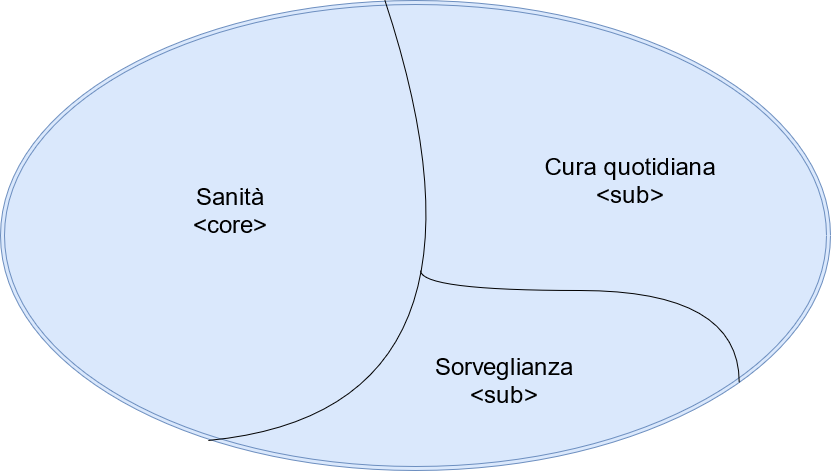
\includegraphics[width=0.5\textwidth]{DrawIo/domainsMap.png}
    \end{figure}
    
    Sono stati identificati tre domain, dove:
    \begin{itemize}
        \item \textbf{Sanità} è il \textbf{core domain}. Contiene tutta la logica e le funzioni utili a determinare lo stato di salute dell'animale, partendo dai soli dati vitali.
        
        \item \textbf{Cura quotidiana} è il \textbf{support domain}. Tramite la cura e le informazioni ricavate dalle azioni quotidiane dell'animale supporta il \textbf{core domain} nell'analisi di anomalie quali patologie, problemi di salute o comportamentali.
        
        \item \textbf{Sorveglianza} è il sub domain relativo alla gestione e monitoraggio video del canile.
    \end{itemize}
    
    \section{Identificazione dei Subdomain}
    Una volta individuato il core-domain, sono emersi anche i domini secondari. %I sottodomini sono stati creati per il replacement piuttosto per il riuso 
    
    %TABELLA SUBDOMAIN
    \begin{figure}[ht]
        \caption{Subdomains}
        \centering
        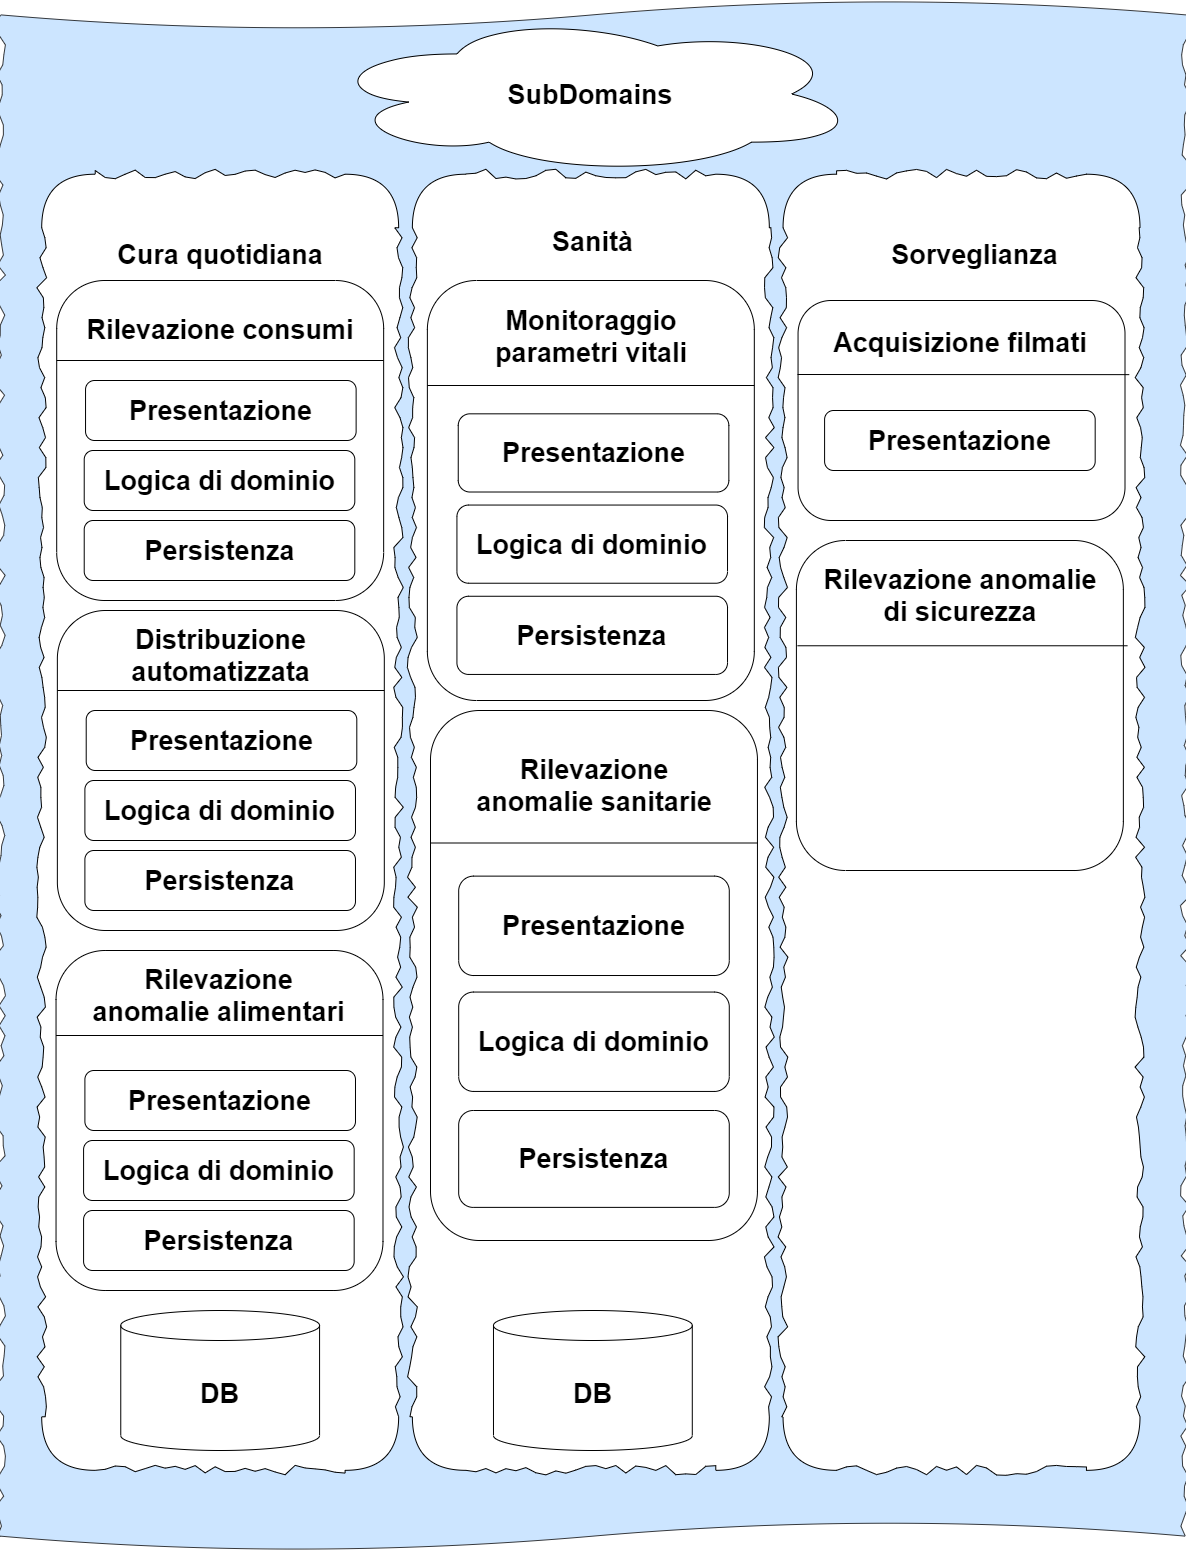
\includegraphics[width=0.9\textwidth]{DrawIo/subDomainsView.png}
    \end{figure}
    
    \section{Definizione dei Bounded Context}
    Un altro importante step è il riconoscimento dei Bounded Contexts. In questa fase il focus è incentrato sul confine tra i moduli individuati in precedenza. Lo scopo è di trovare delle porzioni isolate con confini ben definiti. L’isolamento deve essere non di funzionalità tecnica ma di dominio. Questo paradigma è riconoscibile anche nel trend attuale dei micro-servizi, che, tuttavia sono costruiti attorno ai confini di deployment, non del modello. Ciò assicura l’integrità e la facile scalabilità.
    Il modello del dominio infatti cresce in complessità nel tempo. Questo accade soprattutto nella filosofia Agile che abbraccia il cambiamento. Una continua revisione e raffinamento vengono portati avanti durante tutto l'arco della durata del progetto, per soddisfare differenti business use cases e nuove richieste del cliente. 
    Multipli team che lavorano allo stesso modello, inoltre, possono intralciarsi a vicenda e creare incomprensioni divergenti, a causa delle ambiguità nel linguaggio. 
    Queste sono le sfide avendo un single model, ed è per questo che è meglio avere più contexts/subdomains.
    Nello schema sottostante i Bounded Contexts sono stati collocati, assieme ai SubDomains che li contengono, in base alla loro complessità e alla relativa Business Differentiation. 
    
    %TABELLA BOUNDED CONTEXTS
    \begin{figure}[ht]
        \caption{Bounded Contexts}
        \centering
        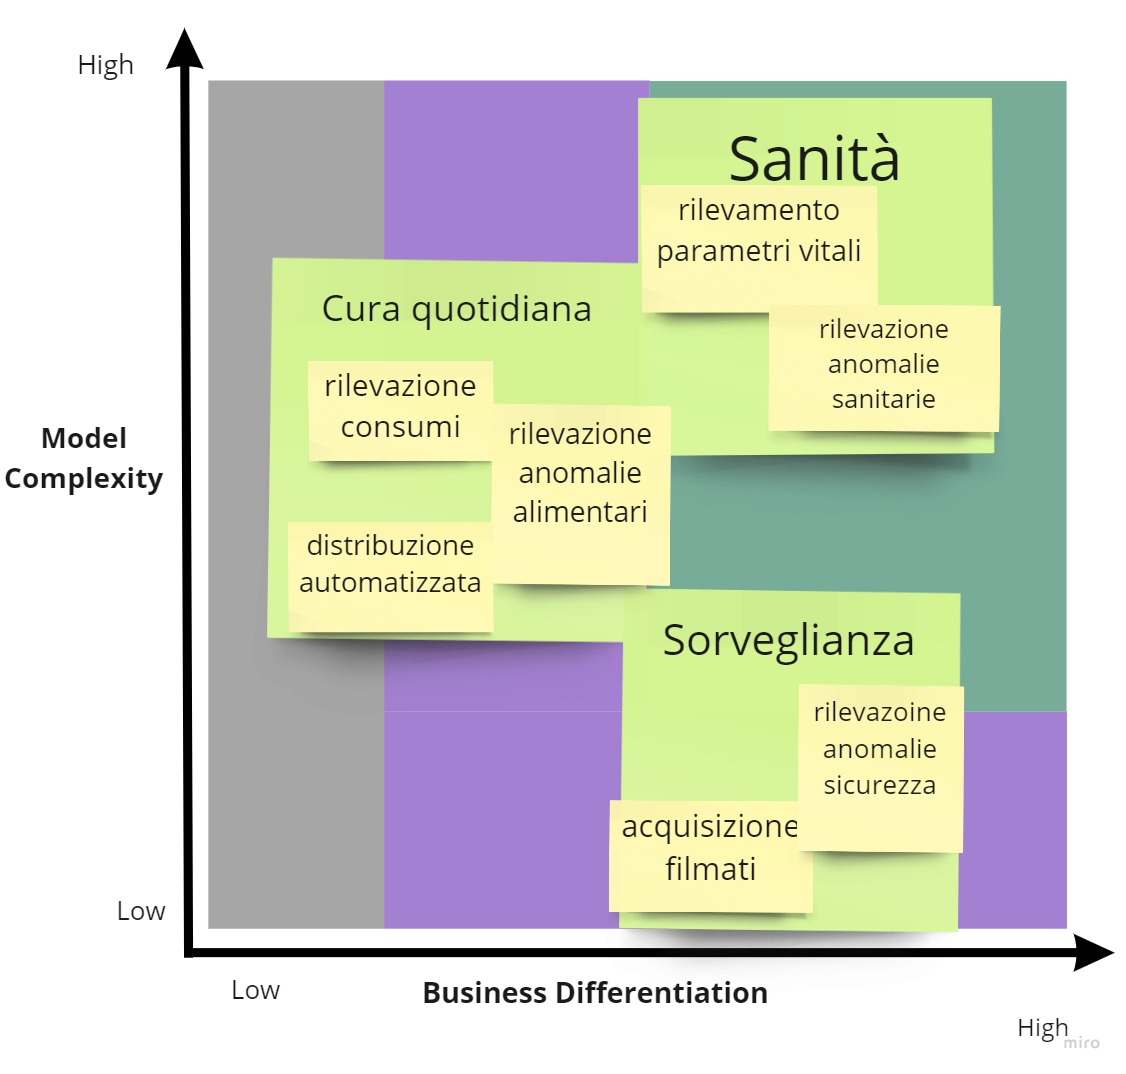
\includegraphics[width=0.9\textwidth]{Miro/BoundedContext.jpg}
    \end{figure}
    
    \section{Definizione delle Context Map}
    %Per creare una context map 
    %Non troppo nel detaglio
    %Descriva lo stato del codice in real-time
    %Mostri i punti di integrazione tra i vari context
    %TABELLA CONTEXT MAP
    \begin{figure}[ht]
        \caption{Context Map}
        \centering
        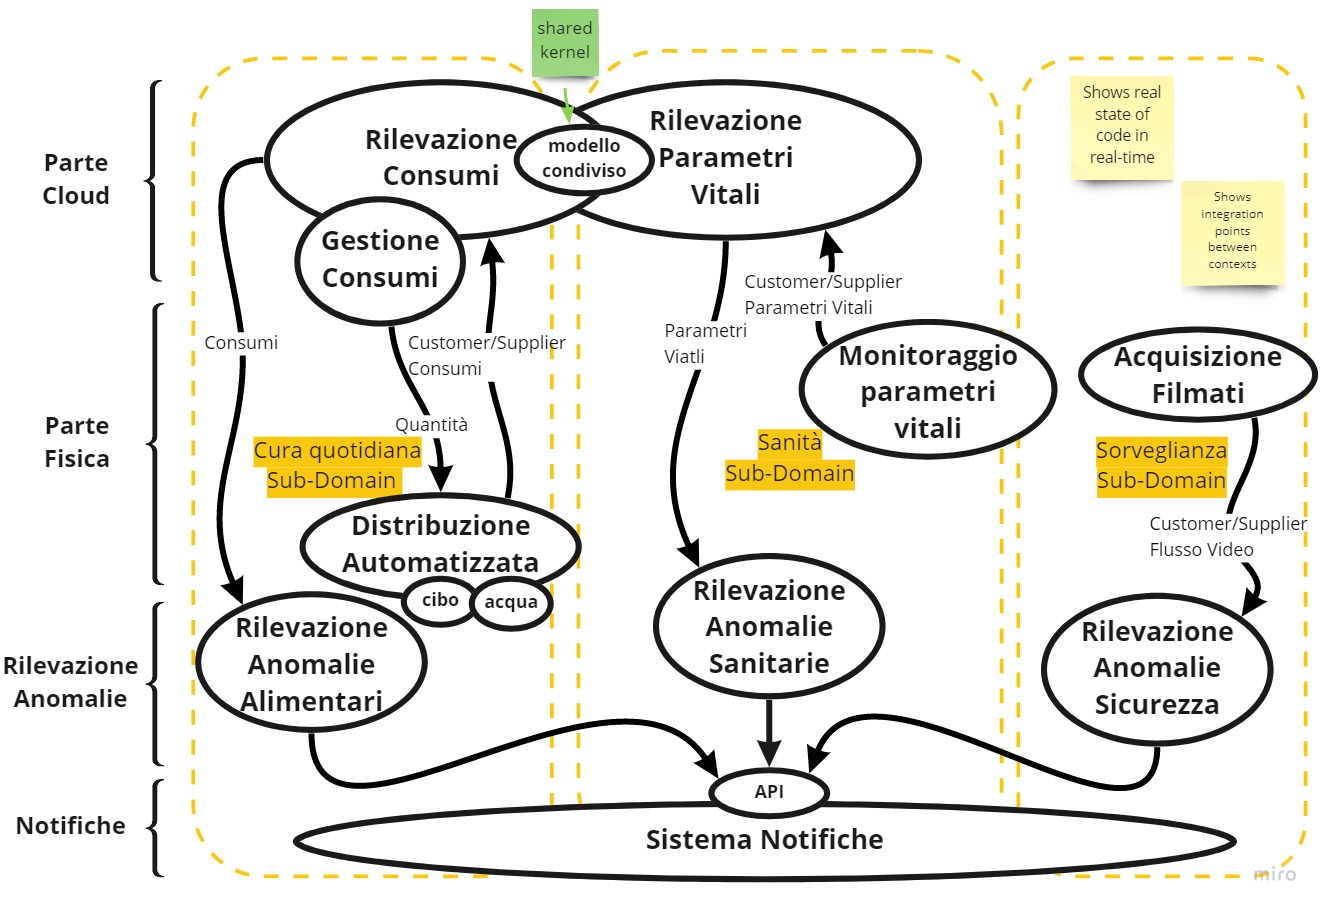
\includegraphics[width=0.9\textwidth]{Miro/ContextMap.jpg}
    \end{figure}
    